\chapter{Corpus study}

\startcontents[chapters]

\section{Methodology}
\subsection{Agreement sources}
The corpus used for this study is the 300M subcorpus of the National Corpus of Polish (NCP 300M), which contains texts from various genres and sources, including fiction, journals, letters, Internet, spoken and educational texts, most of which were created after the year 1990 \citep{przepiorkowski_narodowy_2012}. The corpus was parsed using Trankit \citep{nguyen_trankit_2021} to obtain dependency trees conforming to the Universal Dependencies standard (UD). Those dependency trees were searched for words, which could trigger hybrid agreement: profession nouns, socially gendered nouns and depreciative forms of \textsc{m1} nouns. The dependencies of those words then made it possible to search for attributive agreements (adjectives), predicate agreements (verbs agreeing with their subjects) and relative pronoun agreements. A tagged corpus could have been sufficient for attributive and predicate agreement, but using a parsed corpus gave a better chance of finding the correct relations and agreements within them and made it possible to include relative pronouns in the analysis. The subsections below describe how I chose the nouns for analysis.

\subsubsection{Profession nouns}
Nouns in this category came from two studies about feminitives in Polish. The first was a survey reported by \cite{szpyra-kozlowska_premiera_2019}, where participants were asked to create feminitives from 50 masculine nouns, that in modern Polish do not have feminine counterparts at all or those counterparts are rarely used. For each noun participants had the option to give no answer. The second study was an experiment conducted by \cite{szpyra-kozlowska_czy_2022}, where they tested whether certain feminitives are less accessible by asking participants to try to pronounce them. They chose 20 feminitives, which are formed from masculine nouns that have consonant clusters such as /kt/ (e.g. \textsl{architekt}, meaning 'architect'), /tr/ (e.g. \textsl{geriatra}, meaning 'geriatrician') or /rg/ (e.g. \textsl{chirurg}, meaning 'surgeon'). According to \cite{klemensiewicz_tytuly_1957} adding the -ka suffix, the function of which can be to create the feminitive, makes the word difficult to pronounce. Those two studies give a list of 60 nouns in total, for which it is said to be difficult to form feminine counterparts. It is therefore likely that, if there was a female referent of a noun from this list, the masculine noun would be used, leading to hybrid agreement. 

Both of the studies determine in some way which of the tested nouns have less available feminitives than others: in \cite{szpyra-kozlowska_czy_2022} those are the nouns for which there are the highest error rates in pronunciation, whereas in \cite{szpyra-kozlowska_premiera_2019} -- the nouns for which the most people refused to propose a feminitive. The current study used all of the nouns from those two studies, so as not to set an arbitrary threshold for the qualifying nouns and limit the number of possible agreements for analysis.

Initially, there were 213 070 occurrences of agreement with the 60 nouns in this group. For ease of reference, I call all of the nouns in this category \textsl{profession} nouns, despite not all of them actually referring to professions. Meanings of all nouns are presented in Table \ref{tab:profession}. An example of semantic agreement with a profession noun can be seen in (\ref{ex:prof-occurrence}), where the masculine noun \mean{starosta}{mayor} has a feminine adjective \mean{głogowska}{of Głogów}.

\begin{exe}
  \ex\label{ex:prof-occurrence}
  \gll Na zaproszenie starost-y \sem{głogowsk-iej} Elżbiet-y Urbanowicz - Przysiężn-ej Głogów odwiedziła s. Teresa Jakubowska z ukraińskiego Żytomierza.\\
  on invitation mayor\textsc{(m1)-sg.gen} of.Głogów\textsc{-f.sg.gen} Elżbieta\textsc{-f.gen} Urbanowicz - Przysiężna\textsc{-f.gen} Głogów visited sister Teresa Jakubowska from Ukrainian Żytomierz\\
  \glt ``Invited by the mayor of Głogów, Elżbieta Urbanowicz-Przysiężna, sister Teresa Jakubowska from Żytomierz in Ukraine visited Głogów.''\\
  NCP 300M, sentence ID: 8203800
\end{exe}

\begin{table}[p]
  \centering
  \resizebox{\columnwidth}{!}{
  \begin{tblr}
    {
    vlines, hlines,
    row{1} = {gray9},
    column{1} = {.15\linewidth},
    column{2} = {.35\linewidth},
    column{3} = {.15\linewidth},
    column{4} = {.35\linewidth},
    vline{3} = {1}{-}{},
    vline{3} = {2}{-}{},
    }
    Noun in Polish & Translation or definition in English & Noun in Polish & Translation or definition in English\\
    adiunkt & someone who holds a PhD title and is employed at a scientific institution & architekt & architect\\
    burmistrz & mayor & chirurg & surgeon\\
    demiurg & demiurge & dramaturg & playwright\\
    drań & scoundrel & dupek & asshole\\
    dureń & fool & dziekan & dean\\
    ekspert & expert & elekt & person elected in a specified post, but has not yet entered office\\
    foniatra & phoniatrician & ftyzjatra & pulmonologist\\
    geometra & geometer & geriatra & geriatrician\\
    ginekolog & gynecologist & głupek & fool\\
    herszt & ringleader & inżynier & engineer\\
    jaskiniowiec & caveman & jeniec & captive\\
    jeździec & rider & kierowca & driver\\
    ksiądz & priest & lump & tramp\\
    magister & master (holder of a university degree) & majster & foreman\\
    metalurg & metallurgist & minister & minister\\
    murarz & bricklayer & muzykolog & musicologist\\
    mędrzec & wise man & naukowiec & scientist\\
    nieuk & dunce & nurek & diver\\
    pajac & clown & pastor & pastor\\
    pediatra & pediatrician & petent & applicant\\
    polityk & politician & porucznik & lieutenant\\
    powstaniec & insurgent & prefekt & prefect\\
    premier & prime minister & prezydent & president\\
    proboszcz & parish priest & psychiatra & psychiatrist\\
    pułkownik & colonel & rektor & person in charge of a university\\
    sierżant & sargeant & starosta & highest administrative officer of a second-level unit of local government, mayor\\
    subiekt & salesman & szklarz & glazier\\
    szpieg & spy & szubrawiec & rascal\\
    upiór & phantom & widz & audience member\\
    wójt & highest administrative officer of a basic-level unit of local government, mayor & zbieg & fugitive\\
  \end{tblr}
  }
  \caption{Profession nouns (\textsc{m1}) used in the study, with their translations or definitions in English.}
  \label{tab:profession}
\end{table}

\begin{table}[p]
  \centering
  \begin{tblr}
    {
    vlines, hlines,
    row{1} = {gray9},
    column{1} = {.15\linewidth},
    column{2} = {.1\linewidth},
    column{3} = {.15\linewidth},
    column{4} = {.5\linewidth},
    }
    Noun in Polish & Syntactic gender & Semantic gender & Translation or definition in English\\
    babochłop & \textsc{m2} & feminine & a woman that resembles a man with her physicality, looks and behavior\\
    babol & \textsc{m2} & feminine & a woman that looks or behaves in a way that causes aversion in the speaker\\
    babon & \textsc{m2} & feminine & a woman, about whom the speaker feels negatively\\
    babsko & \textsc{n} & feminine & a woman, about whom the speaker feels negatively\\
    babsztyl & \textsc{m2} & feminine & a woman, about whom the speaker feels negatively\\
    babus & \textsc{m2} & feminine & a woman, about whom the speaker feels negatively\\
    chłopaczysko & \textsc{n} & masculine & a tall or big young man\\
    chłopobaba & \textsc{f} & masculine & a man that resembles a woman with his physicality, looks and behavior (can also mean a woman that resembles a man)\\
    ciota & \textsc{f} & masculine & a homosexual man (can also refer to a woman about whom the speaker feels negatively)\\
    dziewczątko & \textsc{n} & feminine & a girl, whom the speaker likes or to whom they feel compassion\\
    dziewczę & \textsc{n} & feminine & a young girl\\
    dziewuszysko & \textsc{n} & feminine & a girl who causes aversion or contempt in the speaker\\
    kobiecisko & \textsc{n} & feminine & expressively about a woman, augumentative, or to refer to a big woman\\
    kobieciątko & \textsc{n} & feminine & expressively about a woman, diminutive\\
    kobieton & \textsc{m2} & feminine & a woman that resembles a man with her physicality, looks and behavior\\
    pacholę & \textsc{n} & masculine & a boy\\
    pannisko & \textsc{n} & feminine & expressively about a young woman, augumentative\\
    pasztet & \textsc{m3} & feminine & an ugly and unattractive woman\\
    wamp & \textsc{m2} & feminine & a confident, misterious, provocative and attractive woman who seduces men\\
  \end{tblr}
  \caption{Socially gendered nouns used in the study, with their translations or definitions in English.}
  \label{tab:gendered}
\end{table}

\subsubsection{Socially gendered nouns}
I chose the nouns for this category using the Polish Academy of Sciences Great Dictionary of Polish available online.\footnote{https://wsjp.pl/} With the advanced search option, I searched for nouns in the thematic category \textsc{human as a physical being: human physicality: sex}. This search yielded 586 results, which then I filtered manually to find the nouns that only refer to humans (and not, for example, abstract nouns or nouns referring to body parts) and that had incongruent grammatical and semantic gender. There were 19 nouns selected this way: 7 of them were grammatically \textsc{m2} and referred to women (e.g. \textsl{babsztyl}, meaning 'woman' in a pejorative way), 1 was \textsc{m3} and referred to women (\textsl{pasztet}, here meaning a woman whom the speaker finds ugly or unattractive), 7 were grammatically \textsc{n} and referred to women (e.g. \textsl{pannisko}, meaning 'a young woman' in an expressive way), 2 were grammatically \textsc{n} and referred to men (e.g. \textsl{chłopaczysko}, meaning 'a tall or big young man') and 2 were grammatically \textsc{f} and referred to men (e.g. \textsl{ciota}, meaning 'a homosexual man' in a pejorative way). There were 807 occurrences of agreement with those nouns found in the corpus. The full list of nouns in this category with their translations is in Table \ref{tab:gendered}. In (\ref{ex:gend-occurrence}) there is an example of feminine (semantic) agreement on the words \mean{ta}{this} and \mean{ostatnia}{last} with the masculine word \textsl{babsztyl}. Additionally in this examples there are also two words with syntactic agreement with the noun: \mean{groźny}{dangerous} and \mean{odrażający}{offputting}.

\begin{exe}
  \ex\label{ex:gend-occurrence}
  \gll \sem{Ta} \sem{ostatni-a} jest \synt{groźn-ym} i \synt{odrażając-ym} babsztyl-em\\
  this\textsc{(f.sg.nom)} last\textsc{-f.sg.nom} be\textsc{(prs.3sg)} dangerous\textsc{-m1.sg.ins} and offputting\textsc{-m1.sg.ins} woman\textsc{-m1.sg.ins}\\
  \glt ``The last one is a dangerous and offputting woman.''\\
  NCP 300M, sentence ID: 12331643
\end{exe}

\subsubsection{Depreciative forms}
For this category no list of nouns was created, since the corpus was annotated and I could search for the depreciative forms by checking the words' morphological description. It is possible to create depreciative forms of surnames, however these were excluded from the analysis, because there was no way of determining the referents and therefore no way of ensuring that there is hybrid agreement. Surname \textsl{Machała} found in the corpus can serve as an example: let us say that the \textsl{Machała} family bought a new car. Assuming the family consists of at least one man, the speaker can use both (\ref{ex:Machałowie}) and (\ref{ex:Machały}) to convey that information, depending on their attitude they have towards the situation: (\ref{ex:Machałowie}) if the speaker is neutral or positive and (\ref{ex:Machały}) if they are negative. However, if there are only women in the family, the speaker can only use (\ref{ex:Machały}). Without the context it is unclear whether \textsl{Machały} in (\ref{ex:Machały}) is used as a depreciative or simply to refer to women and therefore we cannot decide if this is an example of hybrid agreement.

\begin{exe}
  \ex
  \begin{xlist}
    \ex\label{ex:Machałowie}
    \gll Machał-owie kupi-li nowe auto.\\
    Machała\textsc{(m1)-pl.nom} buy\textsc{-pst.3pl.m1} new car\\
    \ex\label{ex:Machały}
    \gll Machał-y kupi-ły nowe auto.\\
    Machała\textsc{-pl.nom} buy\textsc{-pst.3pl.nm1} new car\\
    \trans ``Machałas bought a new car.''
  \end{xlist}
\end{exe}

Morphological analyzer Morfeusz \citep{kieras_morfeusz_2017} can mark forms as surnames which made it easy to exclude them from the analysis. The other forms marked as depreciative were kept, which gave 254 different lexemes being included as depreciative forms in 1040 agreement occurrences. An example of semantic agreement with a depreciative form can be found in (\ref{ex:depr-occurrence}), where the noun \mean{chłopy}{peasants} in depreciative form has a non-\textsc{m1} ending (\textsl{chłopy} in contrast to the non-depreciative and clearly masculine \textsl{chłopi}), yet still has \textsc{m1} agreement on the word \mean{pomagać}{help}.

\begin{exe}
  \ex\label{ex:depr-occurrence}
  \gll Chłop-y ze wsi \sem{pomaga-li} tutaj.\\
  peasants\textsc{-pl.nom.depr} from countryside helped\textsc{-pst.3pl.m1} here\\
  \glt ``Peasants from the countryside helped here.''\\
  NCP 300M, sentence ID: 9988833
\end{exe}

\subsection{Extracting agreement occurrences from the corpus}
The code used for extracting corpus data in this study can be found in its dedicated GitHub repository.\footnote{https://github.com/bmagdab/hybrid-agreement} The general idea of how the code works is presented in this section.

\subsubsection{Finding the agreement controllers}
After choosing the nouns to be searched in the corpus, it was necessary to find all of their forms and the forms' morphological descriptions, which I did using the morphological analyzer Morfeusz \citep{kieras_morfeusz_2017}. First I searched the corpus for occurrences of nouns, which could be controllers of hybrid agreement. Those nouns were saved if they were in the list of gendered or profession noun forms or if they were marked as depreciative in their morphological description. To ensure that no homonyms were accidentaly saved for later analysis, the morphological description of the found word was compared with the one given by Morfeusz. This way, for example, the word \textsl{premiera} was excluded if it was an instance of the lexeme \mean{premiera}{premiere} in the singular nominative form, but not if it was an instance of the lexeme \mean{premier}{prime minister} in the singular accusative form.

Once the right noun was found, the algorythm searched the dependency tree for words that can agree their gender with that of the noun. This was the head of the noun (which could be an example of predicate agreement), adjectives attached to the noun (which could be examples of attributive agreement), and relative pronouns referring to the noun. Based on the UD annotation guidelines,\footnote{https://universaldependencies.org/workgroups/newdoc/relative\_clauses.html} I searched all dependents of the word for a dependency label with a subtype \textsc{:relcl}, which in the UD annotation scheme marks the head of the relative clause. Then I looked for the dependent of the head of the relative clause, that had a UD feature \textsc{PronType=Rel}, which had to be the relative pronoun.

Using the dependency trees I also automatically annotated the distance between the controller and potential target of agreement (measured in intervening words) and the ordering: whether the target of agreement was the first or not. Once I found the possible agreement targets, I could use the data to look for occurrences of hybrid agreement.

\subsubsection{Extracting and listing agreement occurrences}
To analyse hybrid gender agreement in the found examples, I marked the alternative to the grammatical gender of each agreement controller. For all profession nouns that alternative gender was \textsc{f}, because the only chance of hybrid agreement for those nouns is when the referent is a woman. For socially gendered nouns the alternative gender was assigned depending on the lexeme and for depreciative forms the alternative gender was always \textsc{m1}, because that is the gender of the lexemes that have depreciative forms.

Once I determined the alternative gender, I excluded plural nouns for which the gender discrepancy was between feminine and neuter. This is because for all types of agreement tested here, the plural feminine and plural neuter forms of targets of agreement are syncretic, therefore there is no hybrid agreement in those cases. This happens, for instance, in (\ref{ex:plural-feminine-neuter}), where in singular ((\ref{ex:sg.n}) and (\ref{ex:sg.f})) there is a difference between the feminine and neuter forms of the word \mean{młoda}{young}. In plural (\ref{ex:pl}), however, the form is the same for both neuter and feminine, so hybrid agreement cannot be observed. Examples like this were therefore excluded.

\begin{exe}
  \ex\label{ex:plural-feminine-neuter}
  \begin{xlist}
    \ex\label{ex:sg.n}
    \gll młod-e dziewcz-ę\\
    young\textsc{-n.sg.nom} girl\textsc{(n)-sg.nom}\\
    \ex\label{ex:sg.f}
    \gll młod-a dziewcz-ę\\
    young\textsc{-f.sg.nom} girl\textsc{(n)-sg.nom}\\
    \glt ``young girl''
    \ex\label{ex:pl}
    \gll młod-e dziewcz-ęta\\
    young\textsc{-nm1.pl.nom} girl\textsc{(n)-pl.nom}\\
    \glt ``young girls''
  \end{xlist}
\end{exe}

The next step was to find occurrences of different types of agreement. The predicate agreement of a given noun was found in its head on three conditions: first, dependency label between the noun and the head had to be \textsc{nsubj}, which is the UD label for nominal subjects. Second, the head had to be a verb that inflects for gender, which is only true for verbs annotated as past participles,\footnote{The annotation scheme used for NCP uses the past participle label not only for past participles, but also for parts of past tense and conditional mood forms \citep{przepiorkowski_narodowy_2012}.} active and passive participles. Third, the noun had to be in the nominative case. This condition helps filter out situations where a numeral phrase is in subject position, because then the verb does not agree with the subject -- it is in 3rd person, singular and neuter form, regardless of the noun. Therefore, predicate agreement cannot be observed in those situations at all and they were excluded.

The search was simpler with attributive and relative pronoun agreement. The only requirement for attributive agreement was that the word was an adjective, which was verified by looking for the tag \textsc{adj} in the morphological description of the dependent. As for relative pronouns, all of the ones found earlier were included in the analysis, unless they did not inflect for gender (which was the case, for example, for the word \mean{gdzie}{where}).

In Figure \ref{tree} we can see a sentence from the NCP, which serves as an example of the process of extracting agreement described in this chapter. The word, which can trigger hybrid agreement is \mean{starosta}{mayor}. There are two words in the sentence that agree with this word in terms of gender: \mean{koniński}{of Konin} and \mean{przyznała}{awarded}. All of the information saved for each instance of agreement is shown in Table \ref{tab:extracted-information}.

\begin{figure}[h]
  \centering
  \begin{dependency}
    \begin{deptext}
      Starost-a \& \synt{konińsk-i} \& swój \& puchar \& \sem{przyzna-ła} \& firmie \& Roof \& Reed.\\
      mayor\textsc{(m1)-sg.nom} \& of.Konin\textsc{-m1.sg.nom} \& their \& cup \& awarded\textsc{-pst.3sg.f} \& company \& Roof \& Reed\\
    \end{deptext}
    \deproot{5}{root}
    \depedge{5}{1}{nsubj}
    \depedge{1}{2}{amod}
    \depedge{4}{3}{det:poss}
    \depedge{5}{4}{obj}
    \depedge{5}{6}{iobj}
    \depedge{6}{7}{appos}
    \depedge{7}{8}{flat}
  \end{dependency}
  \caption*{``The mayor of Konin awarded their cup to the company Roof Reed.''}
  \caption{Dependency tree for the sentence from NCP 300M, sentence ID: 10280659.}
  \label{tree}
\end{figure}

% this is from NKJP_300M_102, sentence id: 10280659

\begin{table}[H]
  \centering
\begin{tblr}{
    hline{2-15} = {solid},
    hline{1} = {3-4}{solid},
    vline{3-5} = {solid},
    vline{1-2} = {2-15}{solid},
    cell{3}{1} = {r=5,c=1}{c},
    cell{8}{1} = {r=6,c=1}{c},
    cell{1-2,14}{1} = {c=2}{l},
    cell{2-7}{3} = {c=2}{l},
  }
  & & Occurrence 1 & Occurrence 2 \\
  type of text & & typ\_publ & \\
  source of agreement & form & starosta & \\
  & lexeme & starosta & \\
  & morphological description & subst:sg:nom:m1 & \\
  & grammatical gender & m1 & \\
  & other gender & f & \\
  agreement target & form & przyznała & koniński \\
  & morphological description & praet:sg:f:perf	& adj:sg:nom:m1:pos \\
  & gender & f & m1 \\
  & distance & 3 & 0 \\
  & target first & 0 & 0 \\
  & semantic agreement & 1 & 0 \\
  type of agreement & & predicate & attributive \\
\end{tblr}
\caption{All of the information extracted from the sentence in Figure \ref{tree}}
\label{tab:extracted-information}
\end{table}

\subsubsection{Appositions with profession nouns}
Initial analysis of agreement occurrences with profession nouns showed, that most occurrences cannot be used in this study, because there is no possibility of determining whether the referent of the profession noun is male or female without the context of the surrounding text (sentences were analysed one by one). Because of this I wrote an additional script to extract information about appositions appearing with profession nouns, because if there is a feminine apposition to the profession noun, it is clear that the referent of the noun is female.\footnote{The caveat to this approach is that it is not clear whether the feminine agreement with a profession noun is an occurrence of hybrid agreement, or if the agreement is with the feminine apposition. This is further discussed in the results section.} This is illustrated by example (\ref{ex:prof-occurrence}) from a previous section, repeated here. We can be sure that the \textsc{m1} noun \textsl{starosta} is referring to a woman, because the noun phrase is followed by the full name of the mayor in the same case as the noun phrase.

\begin{exe}
  \exr{ex:prof-occurrence}
  \gll Na zaproszenie starost-y głogowsk-iej Elżbiet-y Urbanowicz - Przysiężn-ej Głogów odwiedziła s. Teresa Jakubowska z ukraińskiego Żytomierza.\\
  on invitation mayor\textsc{(m1)-sg.gen} of.Głogów\textsc{-f.sg.gen} Elżbieta\textsc{-f.gen} Urbanowicz - Przysiężna\textsc{-f.gen} Głogów visited sister Teresa Jakubowska from Ukrainian Żytomierz\\
  \glt ``Invited by the mayor of Głogów, Elżbieta Urbanowicz-Przysiężna, sister Teresa Jakubowska from Żytomierz in Ukraine visited Głogów.''\\
  NCP 300M, sentence ID: 8203800
\end{exe}

The process of extracting information about agreement occurrences is almost identical to what was previously described, only here it applied exclusively to profession noun occurrences and had additional steps to find information about appositions. Using the script I first checked if the dependency head of the profession noun found in the corpus was an apposition. If that was the case, all of the dependents and the head of this apposition were treated as the dependents and the head of the profession noun and I looked for gender agreement between them and the profession noun. I calculated the distance again to make sure it is between them and the profession noun and not the apposition and I saved the word form and the morphological description of the apposition, those fields were left empty if no apposition was found. If the head of the noun was not an apposition, the noun's dependants were searched to see if any of them were an apposition, in which case the procedure described above was performed. This happened in the sentence in (\ref{ex:prof-occurrence}), and we can see the relevant part of the dependency tree in Figure (\ref{starosta-tree}).

\begin{figure}[h]
  \centering
  \begin{dependency}
    \begin{deptext}
      starost-y \& głogowsk-iej \& Elżbiet-y \& Urbanowicz \& - \& Przysiężn-ej\\
      mayor\textsc{(m1)-sg.gen} \& of.Głogów\textsc{-f.sg.gen} \& Elżbieta\textsc{-f.gen} \& Urbanowicz \& - \& Przysiężna\textsc{-f.gen}\\
    \end{deptext}
    \depedge{1}{3}{appos}
    \depedge{1}{2}{amod}
    \depedge{3}{4}{flat}
    \depedge{6}{5}{punct}
    \depedge{4}{6}{conj}
  \end{dependency}
  \caption*{``mayor of Głogów Elżbieta Urbanowicz-Przysiężna''}
  \caption{Dependency tree for a fragment of the sentence in example (\ref{ex:prof-occurrence}).}
  \label{starosta-tree}
\end{figure}

\subsection{Postprocessing of the agreement occurrences}
The 214 917 initial observations were filtered to remove those, which were mistakenly included. There were 263 agreement observations with the gendered \textsc {m3} noun \textsl{pasztet}, which as a gendered noun means a girl or a woman whom the speaker finds unattractive, but it is much more common to use that word to refer to a kind of meat. Most of the occurrences found in the corpus were in that meaning, therefore I removed this noun completely from the study.

Some of the occurrences found had to be parsing mistakes, such as large distances between target and controller, reaching up to 1124 intervening words, relative pronouns preceding the controller and targets of agreements being comprised only of digits, which cannot have any gender agreement marking. All of these were removed.

Another group of occurrences which could not be analysed were acronyms, which were marked as depreciative forms. I removed all of them, because analyzing acronyms is outside of the scope of this study. Similar with targets or controllers of agreement being plural, which could mean that they are a part of a coordination. Coordinate structures are a separate step of Corbett's Agreement Hierarchy and also outside of the scope of this study, so I removed them as well.

Some occurrences were suspicious, because they came from a sentence which had surprisingly many agreements (up to 8). Some of them were not actual sentences, but lists of people with certain functions, for instance a list of mayors chosen in local elections in an area. I looked through sentences with unusually many agreements and removed the ones which were actually lists, since any agreement there was a parsing mistake.

In some occurrences the controller was identified by the parser to have the wrong grammatical gender. This could result in inaccurate calculations of semantic agreement, therefore I also went through them to see what should be corrected and what should be discarded. This way some of the occurrences with the noun \mean{zbieg}{fugitive} were removed, because it was likely that the non-m1 occurrences of this noun were used in a different meaning, for example in the collocation \mean{zbieg okoliczności}{coincidence}. Similarly for the word \mean{upiór}{phantom}, which can also be used to mean a haunting memory, for \mean{lump}{tramp}, which can also mean old, distressed clothing, for \mean{pajac}{clown}, which can also mean a kind of doll and for \mean{nurek}{diver}, which can also refer to the act of diving.

The last part of filtering the data concerned the gender of the target of agreement. Possible values of gendered were predefined: \textsc{m1} or any other with depreciative forms, \textsc{m1} or \textsc{f} with profession nouns and with gendered nouns it depended on the lexeme. There were some occurrences for which the target of the gender was outside of the possible scope, which was most likely a result of parsing mistakes. For depreciative nouns there was no filtering done in this part, for profession nouns I assumed everything but the \textsc{m1} or \textsc{f} agreements was parsing mistakes and removed those occurrences, and for gendered nouns I reviewed the incorrectly marked occurrences manually. 

\subsubsection{Additional processing of profession nouns}
To figure out whether an occurrence of a profession noun referred to a man or a woman, I added information about appositions attached to the nouns. I removed occurrences with plural and non-feminine appositions, because the plural appositions were mostly parsing mistakes and the non-feminine appositions show us that the referent of the noun is not a woman and there cannot be any hybrid agreement, as can be seen in (\ref{ex:prof-appos-m1}), where the noun \textsl{architekt} has a masculine name as an apposition. Since it is possible that in some cases we agree the target with the gender of the apposition and not the gender of the controller, I marked the ordering of the target, controller and apposition for each agreement to be able to look into the influence of the apposition. In (\ref{ex:prof-occurrence}) for example, the order was controller-target-apposition, so it was marked as CTA. Only this selection of 295 occurrences with profession nouns (31 unique lexemes) was saved for further analysis.

\begin{exe}
  \ex\label{ex:prof-appos-m1}
  \gll Dom nasz projektowa-ł mało znany architekt-Ø Stanisław Gądzikiewicz.\\
  house our design\textsc{-pst.3sg.m1} little known architect\textsc{(m1)-sg.nom} Stanisław Gądzikiewicz\\
  \glt ``Our house was designed by a little known architect Stanisław Gądzikiewicz.''\\
  NCP 300M, sentence ID: 24
\end{exe}

\section{Results}
\subsection{Overall results}
The first hypothesis this study aims to test is: there is a monotonous shift from one value of gender to another when going from attributive, through predicate to relative pronoun agreement. Additionally, the hypothesis proposed with the definition of generalized semantic agreement will be tested, which is that split hybrids (here the depreciative forms) are less likely to have generalized semantic agreement than lexical hybrids (here the socially gendered nouns and profession nouns). Before those hypotheses are addressed, we will look at the dataset extracted from the corpus. 

After filtering the data which could not be used, there were 1722 observations, 443 of which were marked as semantic agreement. In Table \ref{tab:corpus-summary} we can see the number of occurrences of agreement for all types of targets (attributes, predicates and relative pronouns) and the percentages of semantic agreement for all those groups. 

\begin{table}[h]
  \centering
  \begin{tblr}
    {
    hlines, vlines,
    row{1,2} = {gray7},
    cell{1}{1} = {r=2}{c},
    cell{1}{2} = {r=2}{c},
    cell{1}{3} = {c=2}{c},
    cell{1}{5} = {c=2}{c},
    hline{6} = {2pt,solid},
    }
    Target of agreement & N & Semantic agreement & & Syntactic agreement & \\
                        & & N & \% & N & \% \\
    Attribute & 891 & 209 & 23.46\% & 682 & 76.54\% \\ 
    Predicate & 686 & 160 & 23.32\% & 526 & 76.68\% \\ 
    Relative pronoun & 145 & 74 & 51.03\% & 71 & 48.97\% \\ 
    Total & 1722 & 443 & 25.73\% & 1279 & 74.27\% \\ 
  \end{tblr}
  \caption{Numbers and percentages of occurrences of agreement with all nouns.}
  \label{tab:corpus-summary}
\end{table}

For statistical modeling of the corpus data I used the \textsl{glmer()} function from the \textsl{lme4} R package. I used binomial logistic regression, because the outcome was binary: whether semantic agreement was chosen or not. The first model used all of the 1722 observations. Fixed effects were the type of agreement target (attribute, predicate or relative pronoun), distance between the target and controller, target placement (preceding or following the controller), type of controller (gendered noun, profession noun or depreciative form) and apposition placement (preceding or following the controller). The corpus contains texts from 13 different types of sources -- this was included as the random effect in the model. The full list of coefficients in this model can be found in Appendix \ref{ap:corpus-coefs} (Table \ref{tab:coef-all}). 

Types of targets and the distance were not significant as predictors of semantic agreement. Target being placed after the controller increased the likelihood of semantic agreement (\textsl{p}<0.001), as well as placing an apposition before the controller (\textsl{p}<0.001). Among the noun types the depreciative forms were the baseline, because the hypothesis was that as split hybrids semantic agreement would be less likely to occurr with them than with the lexical hybrids: gendered and profession nouns. Compared to depreciative forms then, socially gendered nouns turned out to be less likely to have semantic agreement (\textsl{p}<0.001), while profession noun were more likely to have semantic agreement (\textsl{p}<0.001).

Figure \ref{fig:semantic-in-targets} visualises the proportions of semantic and syntactic agreement with different types of agreement, for all nouns combined and for each type of noun separately. The following subsections describe the results for each group of nouns in the study.

\begin{figure}[h]
  \small
  \centering
  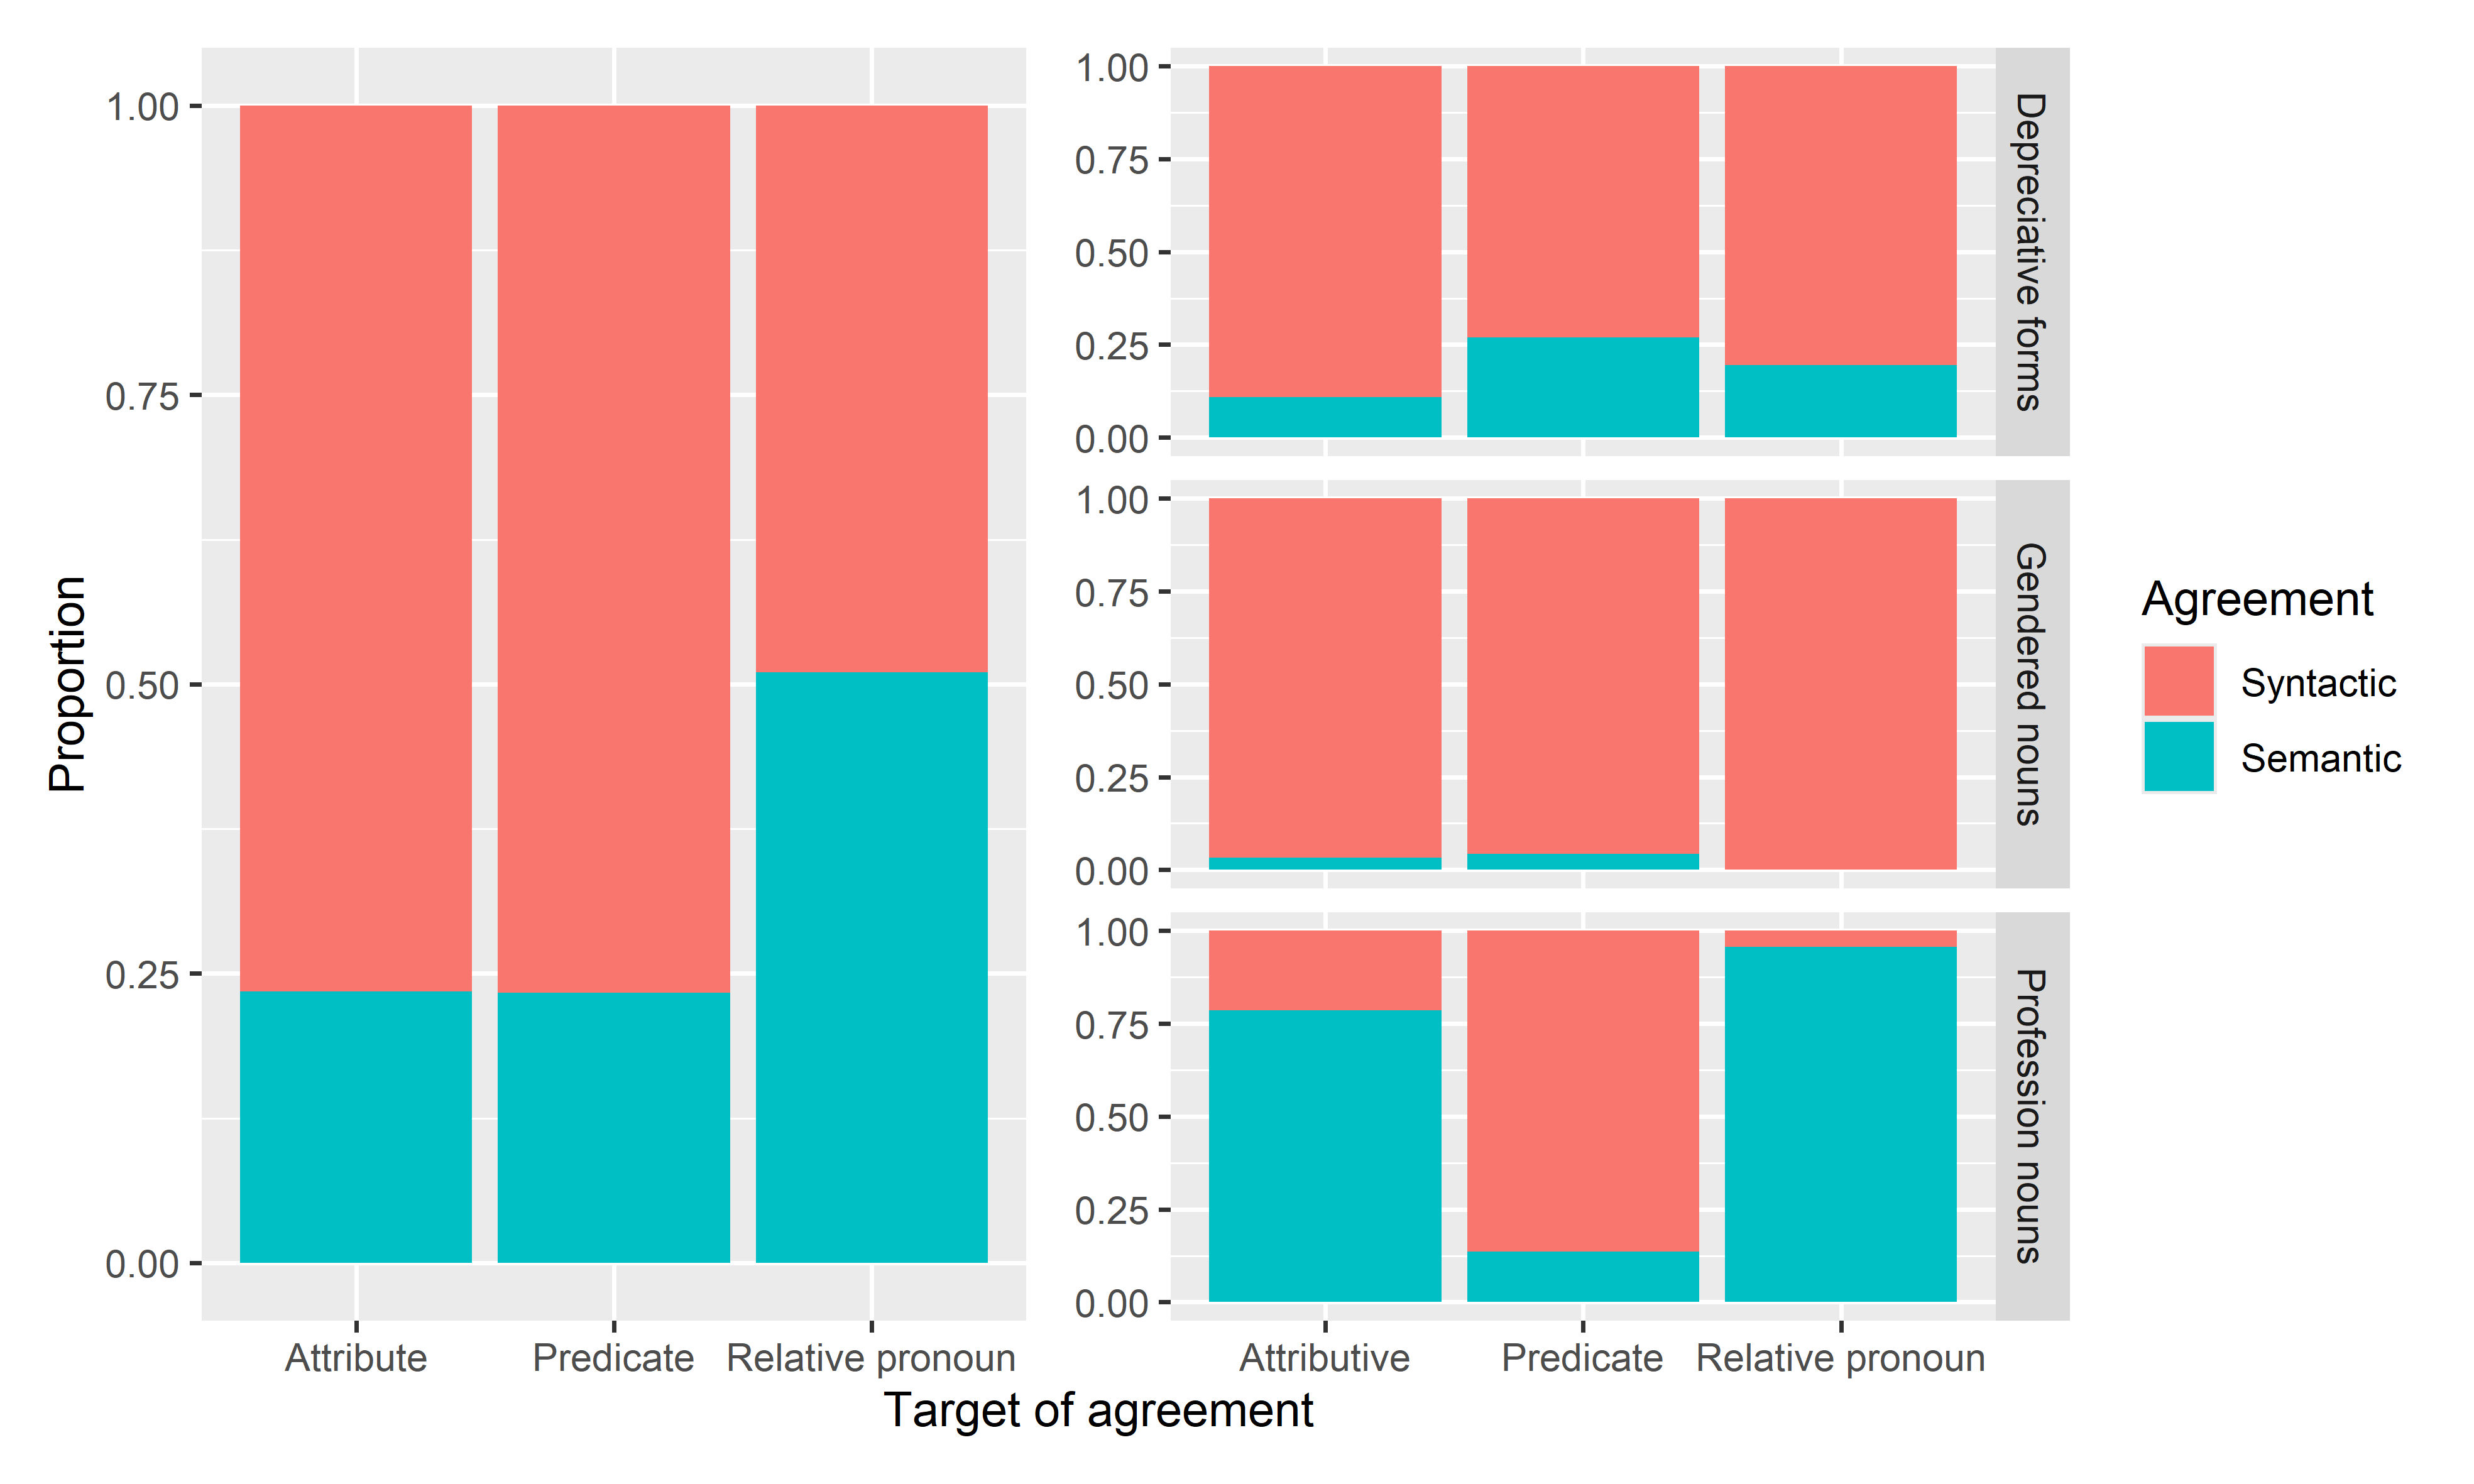
\includegraphics[scale=.7]{images/semXtargetsXnouns.png}
  \caption{Proportions of semantic agreement for each type of target of agreement.}
  \label{fig:semantic-in-targets}
\end{figure}

\subsection{Depreciative forms}
Table \ref{tab:depr-summary} shows the numbers of occurrences and percentages of semantic agreement with depreciative forms. Out of 958 occurrences of agreement with depreciative forms, 20.77\% had semantic agreement. The likelihood of semantic agreement was the lowest for attributes (10.79\%) and highest for predicates (26.89\%), leaving in between the relative pronouns (19.57\%). For this type of controller there is no monotonous change of preference for semantic agreement from attributive to relative pronoun agreement, contrary to Corbett's prediction from the Agreement Hierarchy. 

\begin{table}[H]
  \centering
  \begin{tblr}
    {
    hlines, vlines,
    row{1,2} = {gray7},
    cell{1}{1} = {r=2}{c},
    cell{1}{2} = {r=2}{c},
    cell{1}{3} = {c=2}{c},
    cell{1}{5} = {c=2}{c},
    hline{6} = {2pt,solid},
    }
    Target of agreement & N & Semantic agreement & & Syntactic agreement & \\
                        & & N & \% & N & \% \\
    Attribute & 343 & 37 & 10.79\% & 306 & 89.21\% \\ 
    Predicate & 569 & 153 & 26.89\% & 416 & 73.11\% \\ 
    Relative pronoun &  46 & 9 & 19.57\% & 37 & 80.43\% \\ 
    Total & 958 & 199 & 20.77\% & 759 & 79.23\% \\
  \end{tblr}
  \caption{Numbers and percentages of occurrences of agreement with depreciative forms.}
  \label{tab:depr-summary}
\end{table}

\vspace{-.5cm}
The following examples come from the corpus. We can see that in all of them syntactic agreement was chosen, so in (\ref{ex:depr-attr}) there is syntactic non-\textsc{m1} attributive agreement on the word \textsl{tutejsze} instead of semantic \textsc{m1} \textsl{tutejsi}, in (\ref{ex:depr-pred}) the predicate agreement on \textsl{wolałyby} is syntactic instead of semantic \textsl{woleliby} and in (\ref{ex:depr-relpron}) the relative pronoun is \textsl{które} instead of \textsl{którzy} with semantic agreement. Additionally, in (\ref{ex:depr-sem}) there is an example of semantic predicate agreement.

\begin{exe}
  \ex
  \begin{xlist}
    \ex\label{ex:depr-attr}
    \gll \synt{Tutej-sze} wykształciuch-y nie są polskimi inteligentami.\\
    local\textsc{-nm1.pl.nom} educated.person\textsc{-pl.nom.depr} \textsc{neg} be\textsc{(prs.3pl)} Polish intellectuals\\
    \glt ``The local educated people are not the Polish intellectuals.''\\
    NCP 300M, sentence ID: 12590744\\

    \ex\label{ex:depr-pred}
    \gll Mieszczuch-y \synt{wol-ały-by}, żeby chichotał i mrugał porozumiewawczo.\\
    city.dwellers\textsc{-pl.nom.depr} prefer\textsc{-3pl.nm1-cond} that giggle and wink knowingly\\
    \glt ``The city dwellers would prefer him to giggle and wink knowingly.''\\
    NCP 300M, sentence ID: 3883941\\

    \ex\label{ex:depr-relpron}
    \gll Mnie najbardziej zbijają z nóg modnisi-e, \synt{któ-re} uważają się za orginalne.\\
    me most knock off legs dandy\textsc{-pl.acc.depr} which\textsc{-nm1.pl.nom} consider \textsc{refl} as original\\
    \glt ``Dandys, who consider themselves original, surprise me the most.''\\
    NCP 300M, sentence ID: 6767871\\

    \ex\label{ex:depr-sem}
    \gll Chłopa-ki \sem{pomaga-li} mi przy malowaniu mieszkania.\\
    boy\textsc{-pl.nom.depr} help\textsc{-pst.3pl.m1} me with painting apartment\\
    \glt ``The boys helped me paint the apartment.''\\
    NCP 300M, sentence ID: 5203482
  \end{xlist}
\end{exe}

\vspace{-.5cm}
Table \ref{tab:depr-order} shows semantic agreement for all targets and orderings with depreciative forms. We can see that controller preceding the target has semantic agreement more often than target preceding controller.

\begin{table}[h]
\centering
\begin{tblr}{hlines,vlines}
  Type of target & Target first & Controller first \\ 
  Attributive & 288 (10.07\%) & 55 (14.55\%) \\
  Predicate & 107 (9.35\%) & 462 (30.95\%) \\
  Relative pronoun & -- & 46 (19.57\%) \\
\end{tblr}
\caption{Percentages of semantic agreement for each target and ordering with depreciative forms.}\label{tab:depr-order}
\end{table}

I performed binomial logistic regression using the \textsl{glm()} function from the \textsl{stats} package. The model predicting semantic agreement with depreciative forms based on the type of agreement target, distance and target placement has shown that only target placement had a significant effect on the outcome -- target following the controller increased the likelihood of semantic agreement (\textsl{p}<0.001). The full list of coefficients from this model is in Appendix \ref{ap:corpus-coefs} (Table \ref{tab:coef-depr}).

\subsection{Socially gendered nouns}
According to Corbett's Source Hierarchy, semantic agreement should be more acceptable with lexical hybrids than with split hybrids, which would mean that socially gendered nouns would have a higher percentage of semantic agreements than depreciative forms. As we can see in Table \ref{tab:gend-summary}, this is not reflected in the collected corpus data, where only 3.2\% of occurrences with gendered nouns have semantic agreement. Here the percentages of semantic agreement change monotonously from attributive to relative pronoun agreement, although it is the syntactic agreement that becomes more likely as we go along the Agreement Hierarchy. Considering this, the data from socially gendered nouns fits only the simple constraint of the Agreement Hierarchy \citep{corbett_agreement_2023}. 

\begin{table}[H]
  \centering
  \begin{tblr}
    {
    hlines, vlines,
    row{1,2} = {gray7},
    cell{1}{1} = {r=2}{c},
    cell{1}{2} = {r=2}{c},
    cell{1}{3} = {c=2}{c},
    cell{1}{5} = {c=2}{c},
    hline{6} = {2pt,solid},
    }
    Target of agreement & N & Semantic agreement & & Syntactic agreement & \\
                        & & N & \% & N & \% \\
    Attribute & 343 & 11 & 3.21\% & 332 & 96.79\% \\ 
    Predicate &  95 & 4 & 4.21\% & 91 & 95.79\% \\ 
    Relative pronoun &  31 & 0 & 0\% & 31 & 100\% \\ 
    Total & 469 & 15 & 3.2\% & 454 & 96.8\% \\
  \end{tblr}
  \caption{Numbers and percentages of occurrences of agreement with socially gendered nouns.}
  \label{tab:gend-summary}
\end{table}

The following examples illustrate these agreement preferences. In (\ref{ex:gend-attr}) we can see syntactic attributive agreement in \textsl{stuprocentowa} instead of semantic \textsl{stuprocentowy}, in (\ref{ex:gend-pred}) there is predicate syntactic agreement in \textsl{przytuliło} instead of semantic \textsl{przytuliła} and in (\ref{ex:gend-relpron}) we have \textsl{które} with syntactic agreement instead of \textsl{która} with semantic agreement. Additionally, in (\ref{ex:gend-sem}) there is an example of semantic predicate agreement.

\begin{exe}
  \ex
  \begin{xlist}
    \ex\label{ex:gend-attr}
    \gll Zachichota-ł jak \synt{stuprocentow-a} ciot-a.\\
    giggle\textsc{-pst.3sg.m1} like hundred.percent\textsc{-f.sg.nom} faggot\textsc{(f)-sg.nom}\\
    \glt ``He giggled like a 100\% faggot.''\\
    NCP 300M, sentence ID: 18628964\\

    \ex\label{ex:gend-pred}
    \gll Kobiecisk-o \synt{przytulił-o} się histerycznie do mnie.\\
    woman\textsc{(n)-sg.nom} hug\textsc{-pst.3sg.n} \textsc{refl} histerically to me\\
    \glt ``The woman hugged me histerically.''\\
    NCP 300M, sentence ID: 16919204\\

    \ex\label{ex:gend-relpron}
    \gll Pamiętasz historię dziewczę-cia, \synt{któr-e} uciekło z balu?\\
    remember story girl\textsc{(n)-sg.gen} which\textsc{-n.sg.nom} ran.away from dance\\
    \glt ``Do you remember the story of the girl, who ran away from the dance?''\\
    NCP 300M, sentence ID: 18852664\\

    \ex\label{ex:gend-sem}
    \gll Chłopaczysk-o, gdy go tu niegdyś szukano, \sem{sypia-ł} czas jakiś w kaplicy pogrzebowej.\\
    boy\textsc{(n)-sg.nom} when he here once search sleep\textsc{-pst.3sg.m1} time some in chapel funeral\\
    \glt ``The boy, when once someone was looking for him, slept for some time in the funeral chapel.''\\
    NCP 300M, sentence ID: 17999928
  \end{xlist}
\end{exe}

Table \ref{tab:gend-order} shows that for attributive agreement the controller-first ordering has semantic agreement more often than the target-first ordering, but for predicate agreement it is the other way around.

\begin{table}[h]
\centering
\begin{tblr}{hlines,vlines}
  Type of target & Target first & Controller first \\ 
  Attributive & 290 (2.76\%) & 53 (5.66\%) \\
  Predicate & 28 (7.14\%) & 67 (2.99\%) \\
  Relative pronoun & -- & 31 (0\%) \\
\end{tblr}
\caption{Percentages of semantic agreement for each target and ordering with socially gendered nouns.}\label{tab:gend-order}
\end{table}

Binomial logistic regression (performed with the \textsl{glm()} function from the \textsl{stats} package) using only the agreement occurrences with socially gendered nouns with the type of agreement target, distance and target placement as predictors has shown that distance was the only significant predictor of semantic agreement: larger distance increased the likelihood of semantic agreement with gendered nouns (\textsl{p}<0.05). The full list of coefficients from this model can be found in Appendix \ref{ap:corpus-coefs} (Table \ref{tab:coef-gend}).

\subsection{Profession nouns}
As we can see in Table \ref{tab:prof-summary}, there were 295 occurrences of agreement with profession nouns, 77.63\% of which had semantic agreement. This percentage is larger than for other types of nouns, however this is most likely because all of the profession noun occurrences included in the analysis appeared with feminine appositions, which increase the likelihood of semantic agreement. I will explore this more later when considering the order in which the apposition, controller and target appear in the sentences. With profession nouns it was more likely that semantic agreement would be used in attributes (78.54\% of all attributive agreement occurrences) and in relative pronouns (95.59\% of all relative pronoun agreement occurrences), but not in predicates (13.64\% of all predicate agreement occurrences). This, again, does not follow the simple constraint of the Agreement Hierarchy proposed by Corbett (2023), according to which there should be a monotonic change from attributive to relative pronoun agreement. 

\begin{table}[H]
  \centering
  \begin{tblr}
    {
    hlines, vlines,
    row{1,2} = {gray7},
    cell{1}{1} = {r=2}{c},
    cell{1}{2} = {r=2}{c},
    cell{1}{3} = {c=2}{c},
    cell{1}{5} = {c=2}{c},
    hline{6} = {2pt,solid},
    }
    Target of agreement & N & Semantic agreement & & Syntactic agreement & \\
                        & & N & \% & N & \% \\
    Attribute & 205 & 161 & 78.54\% & 44 & 21.46\% \\ 
    Predicate &  22 & 3 & 13.64\% & 19 & 86.36\% \\ 
    Relative pronoun &  68 & 65 & 95.59\% & 3 & 4.41\% \\ 
    Total & 295 & 229 & 77.63\% & 66 & 22.37\% \\
  \end{tblr}
  \caption{Numbers and percentages of occurrences of agreement with profession nouns.}
  \label{tab:prof-summary}
\end{table}

The examples below illustrate the agreement preferences visible in Table \ref{tab:prof-summary}. Attributive agreement in (\ref{ex:prof-attr}) is semantic on the word \textsl{obecnej} instead of syntactic \textsl{obecnego}, the predicate agreement in (\ref{ex:prof-pred}) is the syntactic \textsl{zapewniał} instead of semantic \textsl{zapewniała} and the relative pronoun agreement in (\ref{ex:prof-relpron}) is the semantic \textsl{która} instead of syntactic \textsl{który}.

\begin{exe}
  \ex
  \begin{xlist}
    \ex\label{ex:prof-attr}
    \gll Większość złożyli w końcówce kadencji \sem{obecne-j} burmistrz-Ø Stefanii Sulińskiej.\\
    majority submitted in ending term current\textsc{-f.sg.gen} mayor\textsc{(m1)-sg.nom} Stefania Sulińska \\
    \glt ``The submitted the majority of them at the end of the term of the current mayor, Stefania Sulińska.''\\
    NCP 300M, sentence ID: 10793552\\

    \ex\label{ex:prof-pred}
    \gll One są gotowe do adaptacji do roku 2008 – \synt{zapewniał-Ø} minist-er edukacji Krystyna Łybacka.\\
    they are ready for adaptation to year 2008 - assured\textsc{-pst.3sg.m1} minister\textsc{(m1)-sg.nom} education Krystyna Łybacka\\
    \glt ``They are ready to be adapted before the year 2008 - assured the minister of education Krystyna Łybacka.''\\
    NCP 300M, sentence ID: 4040070\\

    \ex\label{ex:prof-relpron}
    \gll Felicity Huffman gra panią naukow-iec, \sem{któr-a} w arktycznej stacji zostaje zarażona pasożytem z kosmosu.\\
    Felicity Huffman plays lady scientist\textsc{(m1)-sg.nom} which\textsc{-f.sg.nom} in arctic station becomes infected parasite from space\\
    \glt ``Felicity Huffman plays the scientist, who is infected with a parasite from space in the arctic station.''\\
    NCP 300M, sentence ID: 18469406\\
  \end{xlist}
\end{exe}

In Table \ref{tab:prof-order} we can see that for attributive agreement the target-first ordering has semantic agreement more often than the controller-first ordering, in contrast to predicate agreement, where the controller-first ordering has semantic agreement more often.

\begin{table}[h]
\centering
\begin{tblr}{hlines,vlines}
  Type of target & Target first & Controller first \\ 
  Attributive & 186 (80.65\%) & 19 (57.89\%) \\
  Predicate & 8 (12.5\%) & 14 (14.29\%) \\
  Relative pronoun & -- & 68 (95.59\%) \\
\end{tblr}
\caption{Percentages of semantic agreement for each target and ordering with profession nouns.}\label{tab:prof-order}
\end{table}

It is possible that agreement with profession nouns is more likely to be semantic than with other types of nouns, because in those occurrences there were also feminine appositions to the nouns (which were necessary, because without them it would be impossible to tell in corpus examples whether the noun referes to a woman or not). In those situations it is possible that speakers chose feminine agreement on targets (which for profession nouns is semantic agreement), because they were actually agreeing the gender of the target with the gender of the apposition. To have more insight into the structure of those sentences I marked the order in which the appositions (A), controllers (C) and targets (T) appeared with each occurrence of agreement. Figure \ref{fig:ordering} shows the proportions of semantic to syntactic agreement in occurrences with each possible order of appositions, controllers and targets.

\begin{figure}[h]
  \centering
  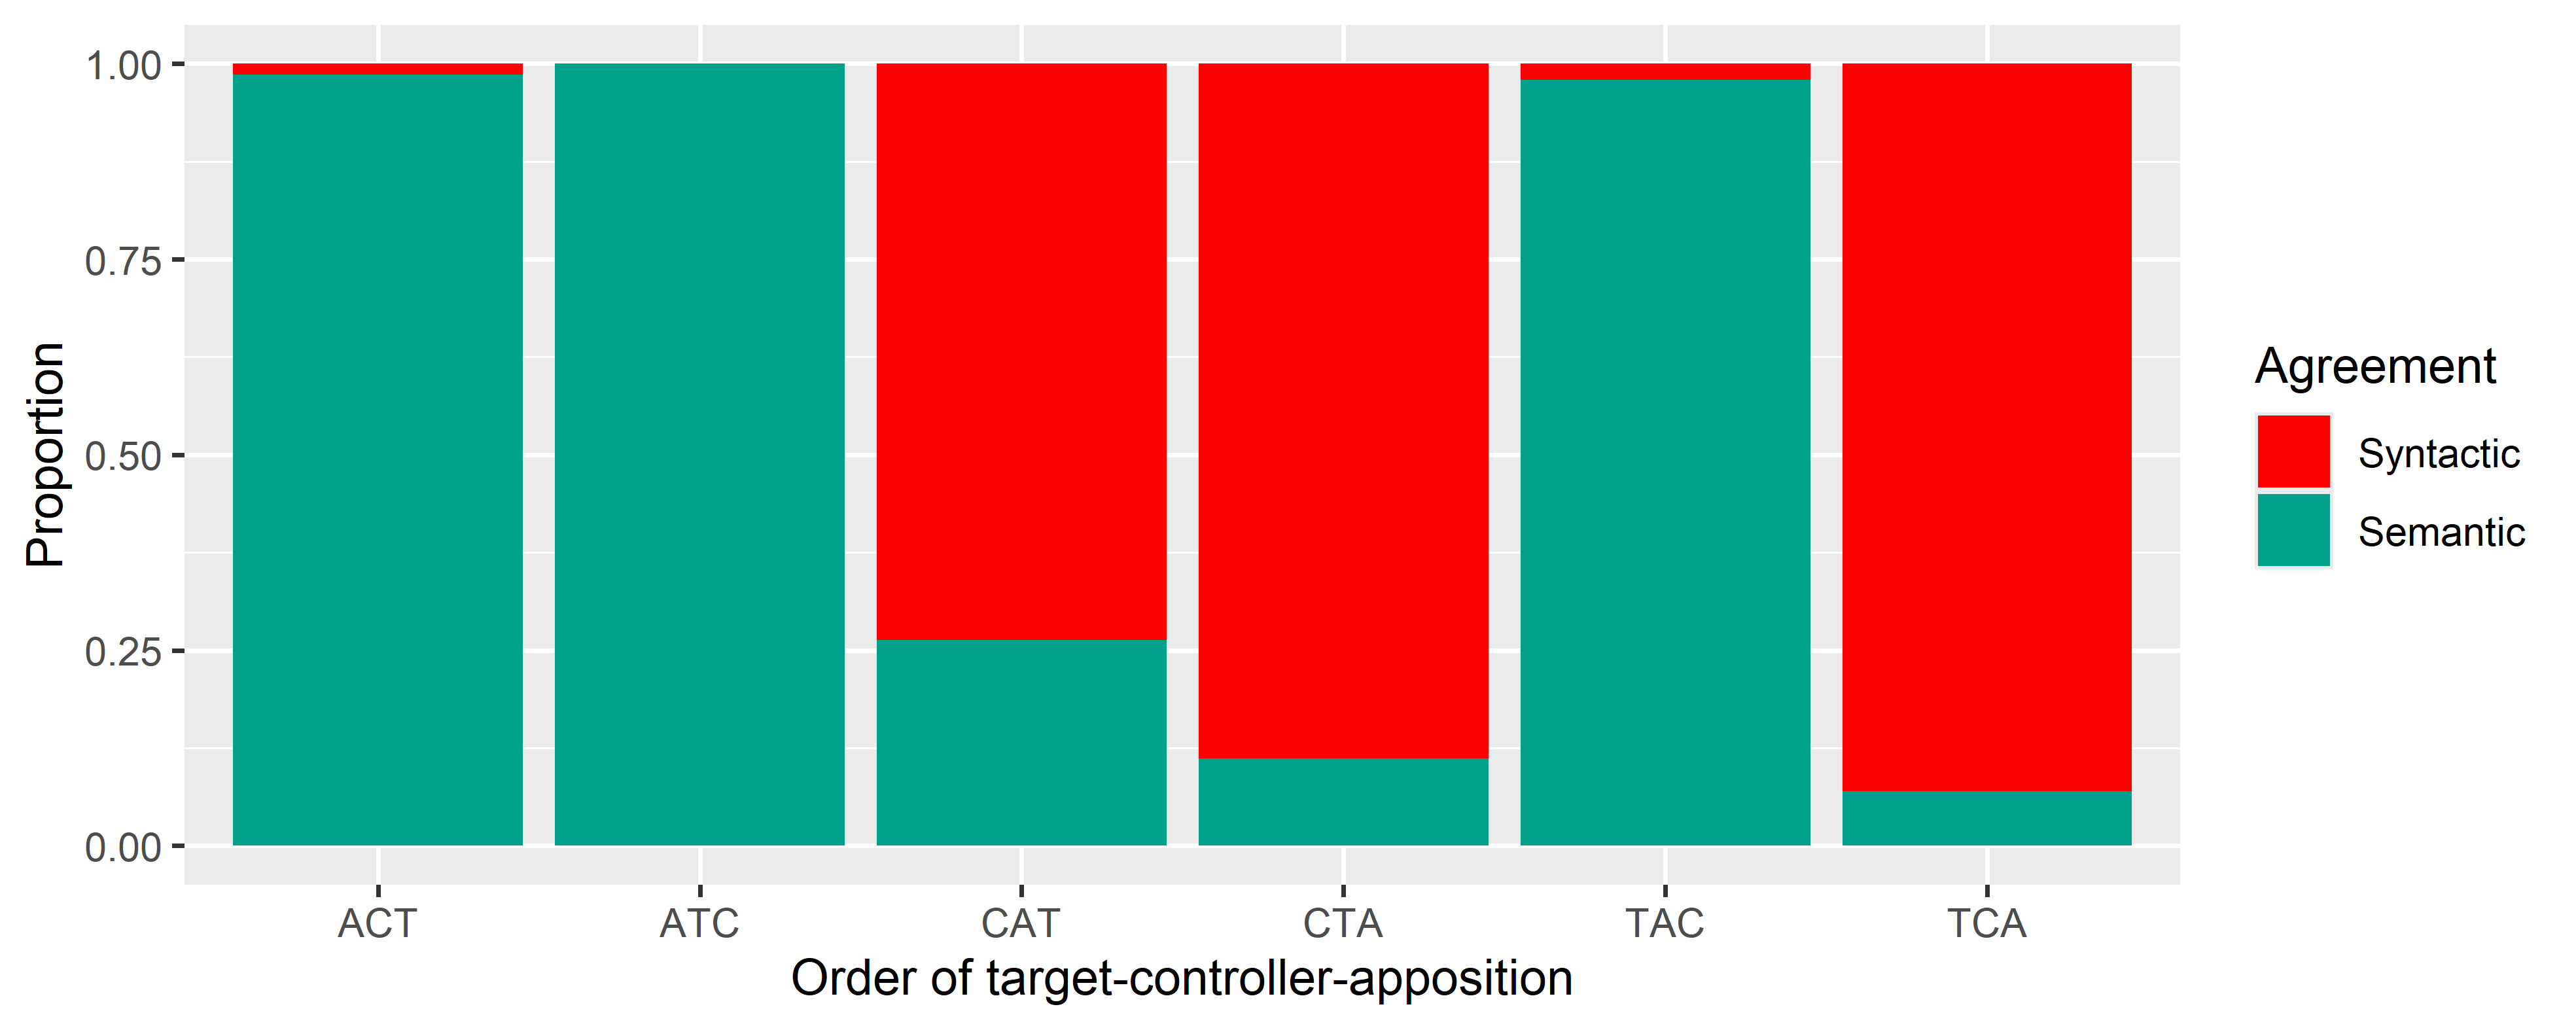
\includegraphics[width=\linewidth]{images/semXorder.png}
  \caption{Proportion of syntactic and semantic agreements with ordering of the controller, target and apposition}
  \label{fig:ordering}
\end{figure}

Three of the orders shown in the figure noticeably favor semantic agreement over syntactic: apposition-controller-target, apposition-target-controller and target-apposition-controller. In contrast to the other orders, for these the apposition appears before the controller. Since this seems to be the most important information coming from the order variable, for statistical modeling instead of accounting for the order  we will account for whether the apposition appears first (before the controller) or not.

For statistical modeling I used the \textsl{glm()} function from the \textsl{stats} package. The binomial logistic regression performed on agreement occurrences with profession nouns used the type of agreement target, distance, target placement and apposition placement as predictors of semantic agreement. Distance and target placement were not significant in this model. Contrary to what the Agreement Hierarchy indicates, the odds of attributive agreement being semantic were approximately 16.16 times higher than the odds of predicate agreement being semantic (\textsl{p}<0.05). For relative pronouns the odds were 25.84 times higher than for predicates (\textsl{p}<0.05). There was also a significant effect of apposition placement -- the apposition appearing before the controller increased the likelihood of semantic agreement (\textsl{p}<0.001). The full list of coefficients from this model is in Appendix \ref{ap:corpus-coefs} (Table \ref{tab:coef-prof}).

\begin{table}[H]
  \centering
  \begin{tblr}
    {
    hlines, vlines,
    row{1,2} = {gray7},
    cell{1}{1} = {r=2}{c},
    cell{1}{2} = {r=2}{c},
    cell{1}{3} = {c=2}{c},
    cell{1}{5} = {c=2}{c},
    hline{6} = {2pt,solid},
    }
    Target of agreement & N & Semantic agreement & & Syntactic agreement & \\
                        & & N & \% & N & \% \\
    Attribute &  46 & 3 & 6.52\% & 43 & 93.48\% \\ 
    Predicate &  19 & 3 & 15.79\% & 16 & 84.21\% \\ 
    Relative pronoun &   6 & 3 & 50\% & 3 & 50\% \\ 
    Total &  71 & 9 & 12.68\% & 62 & 87.32\% \\ 
  \end{tblr}
  \caption{Numbers and percentages of occurrences of agreement with profession nouns without occurrences with appositions first.}
  \label{tab:prof-sum-NOAPP}
\end{table}

Considering the effect of apposition placement on the choice of agreement, we can look at how the proportions of semantic agreement change if we exclude occurrences with apposition first, because the speakers agree the gender of the target with the gender of apposition and not the semantic gender of the controller. Table \ref{tab:prof-sum-NOAPP} is identical to Table \ref{tab:prof-summary} and figure \ref{fig:NOAPP-semantic-in-targets} is identical to Figure \ref{fig:semantic-in-targets}, only with occurrences of profession nouns with appositions first excluded.

\begin{figure}[H]
  \small
  \centering
  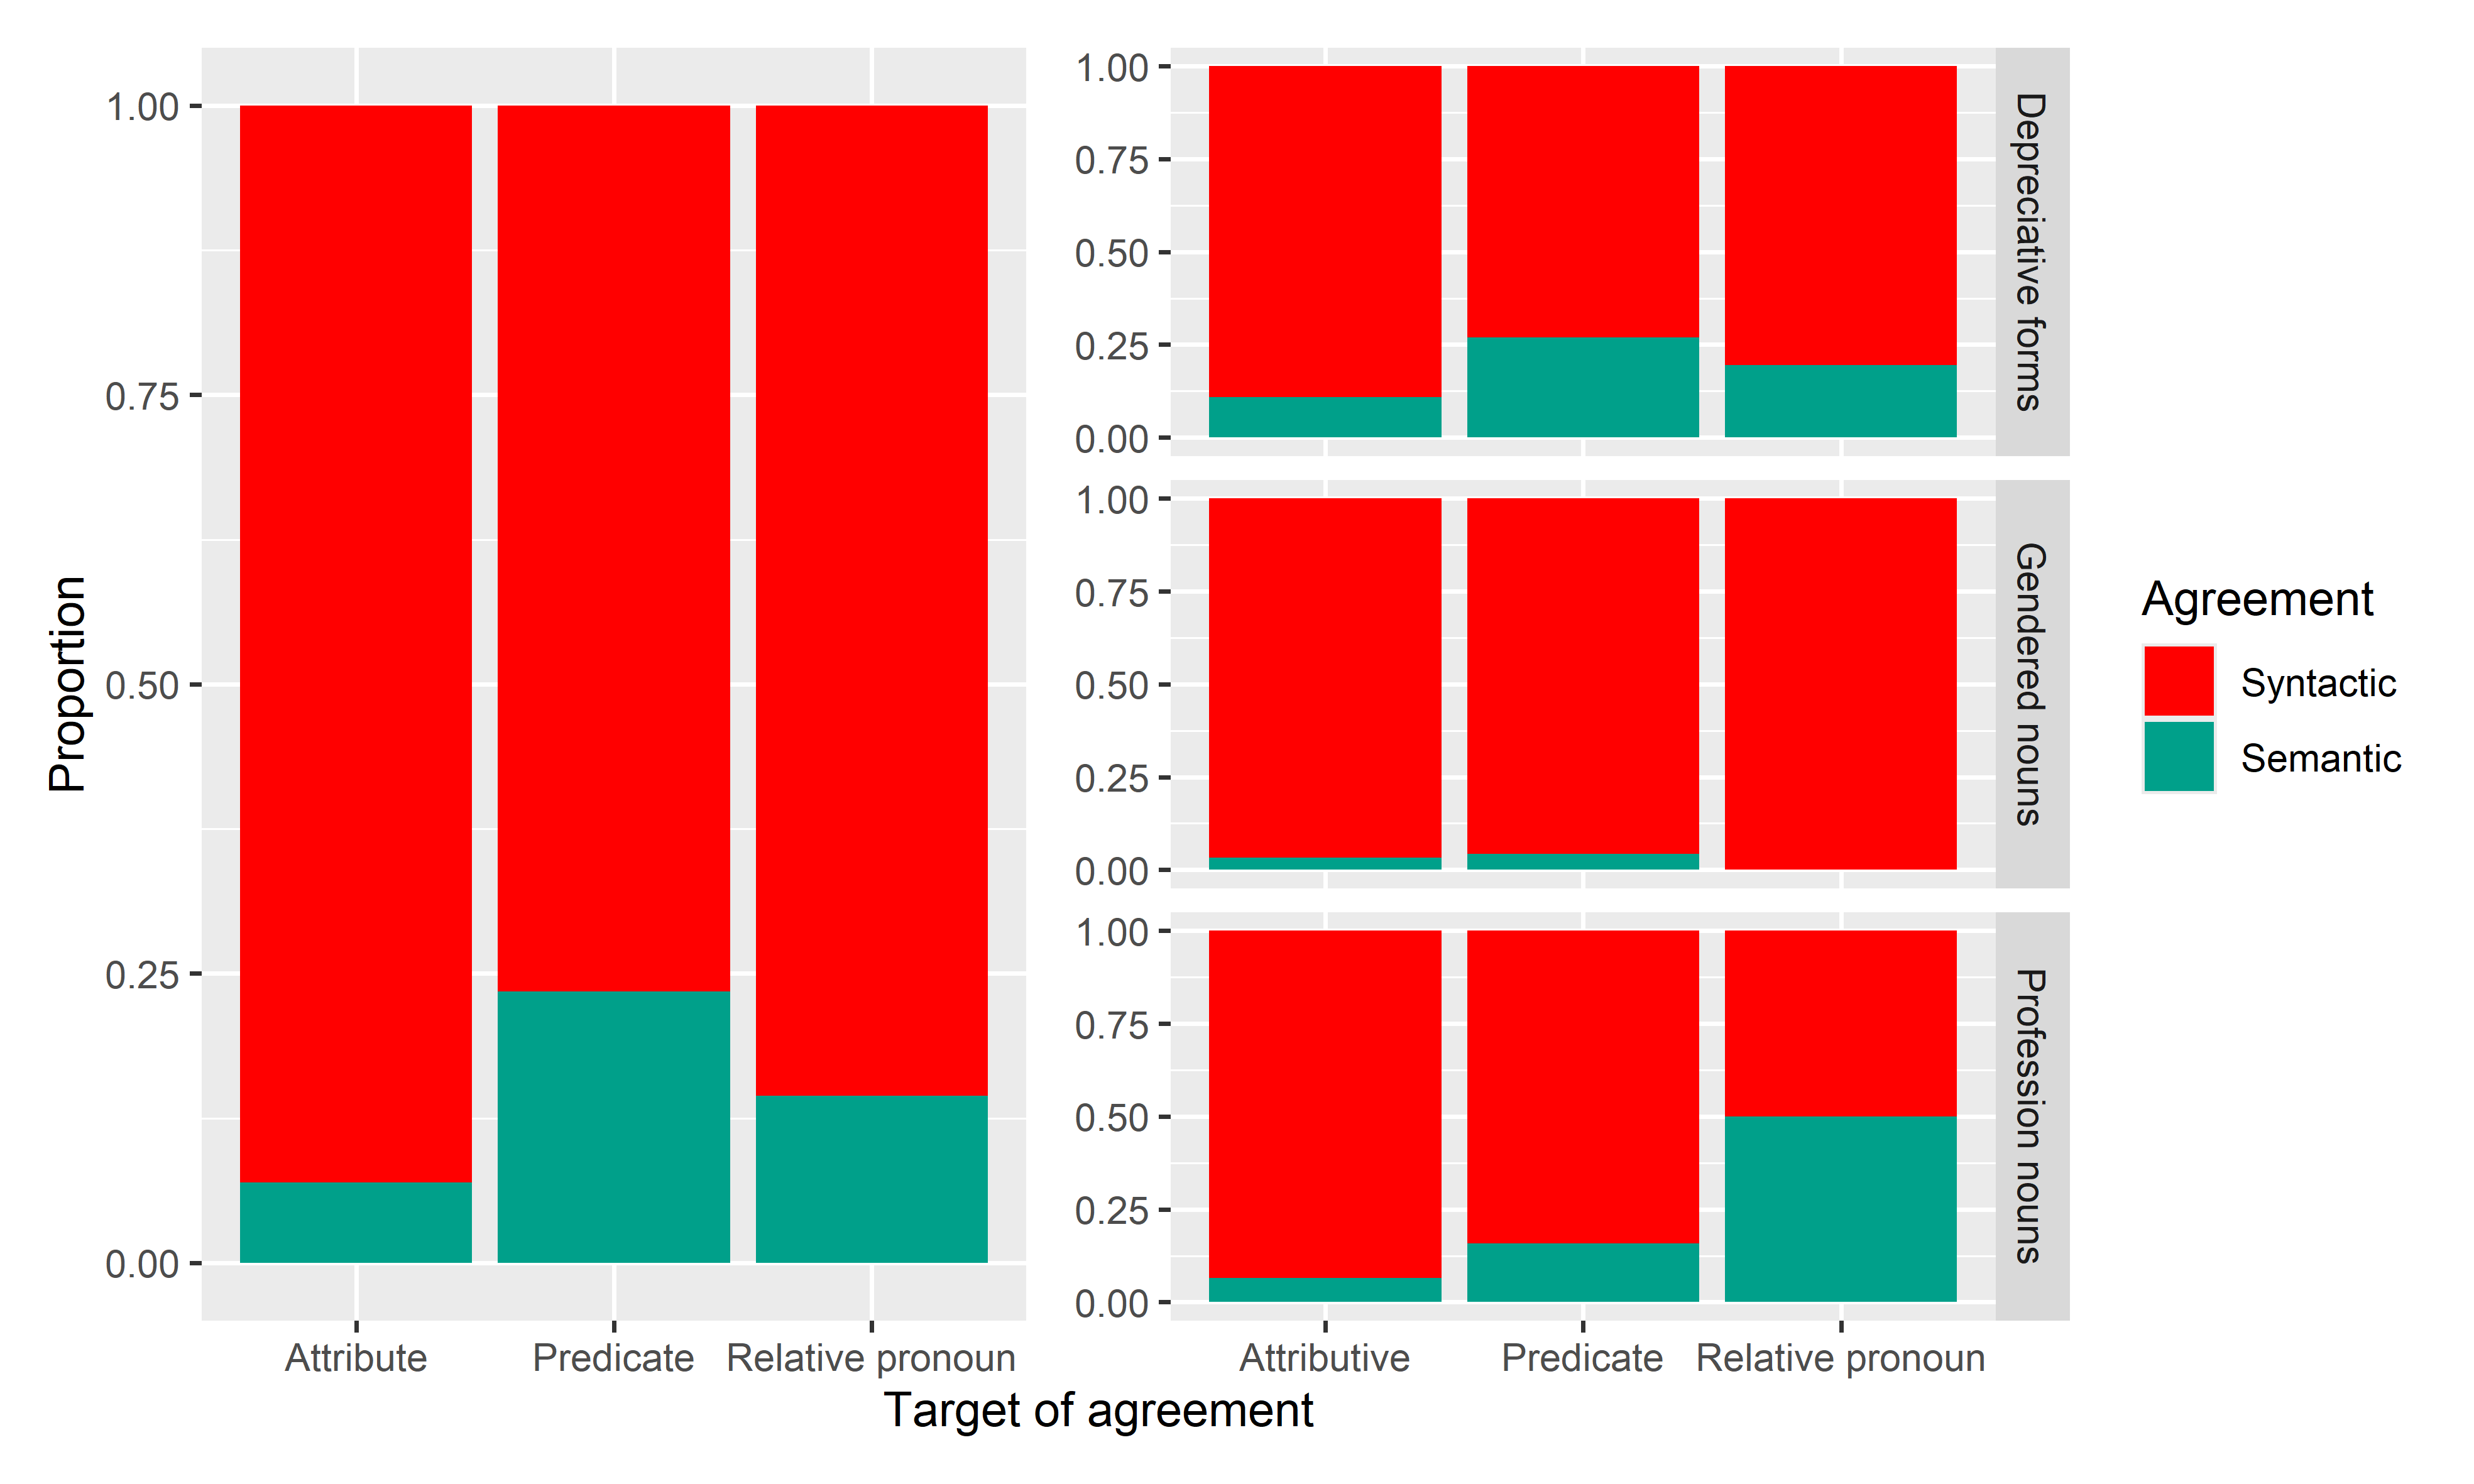
\includegraphics[width=\linewidth]{images/NOAPPsemXtargetsXnouns.png}
  \caption{Proportions of semantic agreement for each type of target of agreement without occurrences of profession nouns with preceding appositions.}
  \label{fig:NOAPP-semantic-in-targets}
\end{figure}

\vspace{-.5cm}
We can see that the overall proportions of semantic agreement (left side of the figure) are now unambiguously not monotonic, and therefore not compatible with any version of the Agreement Hierarchy constraints. The proportions for the profession nouns only, however, now show a monotonic shift from preference for almost exclusively syntactic agreement with attributes, to close to 50\% syntactic and semantic agreement. 

\vspace{-.5cm}
\section{Discussion}
When looking at all nouns combined, there was a clear preference for syntactic agreement (74\% of all occurrences) and no significant effect of the type of target or the distance between the target and the controller. Instead, the choice between semantic and syntactic agreement could be better predicted with the order of target and controller, the type of noun and the apposition -- whether it was there and whether it preceded the agreement controller. This is a surprising result, because the type of agreement target was hypothesised to be the main factor in the choice between semantic and syntactic agreement. 

As for the effect of the type of noun, based on the Hierarchy of Agreement Sources, the lexical hybrids (profession nouns and socially gendered nouns) should be more likely to have semantic agreement than split hybrids (depreciative forms). There is a significant difference between the lexical hybrids and split hybrids, but it goes in different directions: socially gendered nouns are less likely to have semantic agreement than depreciative forms, while profession nouns are more likely to have semantic agreement than depreciative forms. Looking at this, it is inconclusive whether the lexical hybrids are more likely to have semantic agreement. However, if we exclude the profession nouns with appositions preceding the agreement controllers, we see that only 12.68\% of all agreement occurrences are semantic, compared to 20.77\% for depreciative forms. It is possible that when appositions precede the controllers, gender of targets is actually agreed with the appositions, and in this case all lexical nouns in this study have less semantic agreement than depreciative forms.

Within the depreciative forms, the only significant factor was the ordering of target and controller: target following the controller increased the likelihood of semantic agreement. This is in line with the hypothesis about the target and controller order.

Among the agreement occurrences with socially gendered nouns there is barely any semantic agreement. One reason for this could be the source of occurrences with those nouns: over 50\% of those occurrences come from literature, which can be highly stylized and can affect the choice of agreement with those nouns. 

Profession nouns are the only group, for which the type of agreement target was a significant predictor of semantic agreement, but not in the way the Agreement Hierarchy predicts -- attributive agreement was more likely to be semantic than predicate agreement. In Figure \ref{fig:NOAPP-semantic-in-targets} we can see however, that if we exclude the profession noun occurrences with appositions preceding the controller, the proportion of semantic agreement changes monotonically with the smallest in attributive agreement and the largest in relative pronoun agreement. There is the possibility that with apposition preceding the controller of agreement causes speakers to choose the target gender based on the apposition and not on the controller. This seems more likely when we look at the proportions of semantic agreement in Figure \ref{fig:ordering} and take into account that apposition placement was a significant predictor of semantic agreement in both the general and the profession nouns model -- for profession nouns only when a feminine apposition appears before the controller it is 63\% more likely that there will be semantic agreement, than if the apposition was after the controller.

The main limitation here was that it was a corpus study, therefore it was impossible to control for the variables of interest. There was little data for socially gendered nouns and a lot for profession nouns, which had to be heavily filtered to be included in the analysis. Even the filtering was not fully satisfactory, since the profession noun occurrences had to have appositions included to make sure that there was in fact hybrid agreement. This in turn causes the interpretation of profession noun results to be unclear.

To continue the research on hybrid agreement in Polish, I decided to conduct two acceptability judgement experiments. I decided to use profession nouns and depreciative forms, so that it is possible to reach more definite conclusions regarding the profession nouns, and so that there is more data about split hybrids, which are a newer and less explored addition to the agreement hierarchy. The experimental study allows me to control the context, so that there is no need for using appositions and it is clear that gender agreement on the target comes from the controller.
